\section{Goal of the experiment}
In this experiment, the process of optical pumping will be used to precisely measure properties of Rubidium atoms such as the hyperfine constant $A$ via absorption measurements. In addition to that, relaxation times of the induced pumped states as well as external magnetic fields will also be measured by observing the effect of magnetic fields, applied through Helmholtz coils, high frequency radio waves and variations in the laser intensity.
\section{Physical principles}
\subsection{Hyperfine structure and Zeeman splitting}
This section is based on the detailed elaborations in \cite{staatsex}.\\
The fine structure levels of the atomic spectrum, which splits the basic levels into sub-levels due to spin-orbit interaction, can be shown to be split into even finer levels, whose energetic distances are roughly three orders of magnitude smaller than those of the fine structure. This is called the 'hyperfine structure' and is mainly caused by the interaction of the nuclear magnetic dipole and quadrupole moment and the magnetic field of the shell electrons. Its structure for the two Rubidium isotopes that are used in this experiment can be seen in figure \ref{fig:hyperfinestructure}.\\

As the nucleus is charged and, expressed as the nuclear spin $\vec{I}$, has angular momentum, it also has a magnetic moment, which is $\vec{\mu}_I=\frac{g_I\mu_K}{\hbar}\vec{I}$, where $g_I$ is the g-factor of the nucleus and $\mu_K$ is the nuclear magneton. 

With the total angular momentum of the electrons $\vec{J}$, the total angular momentum of the atom can be written as

\begin{equation}
\vec{F}=\vec{J}+\vec{I},\qquad \lvert I-J\rvert\le F \le I+J
\end{equation}

The energy difference between hyperfine structure levels can then shown to be

\begin{equation}
\Delta E_{HFS}=-\vec{\mu}_I\cdot\vec{B}_J=\frac{A}{2}(F(F+1)-J(F+1)-I(I+1))
\end{equation}

where $A=\frac{g_I\mu_KB_J}{\sqrt{J(J+1)}}$ is the hyperfine constant. Neighboring levels thus have an energy difference of

\begin{equation}
\Delta E_{HFS}(F+1)-\Delta E_{HFS}(F)=A(F+1)
\end{equation}

\begin{figure}[H]
\centering
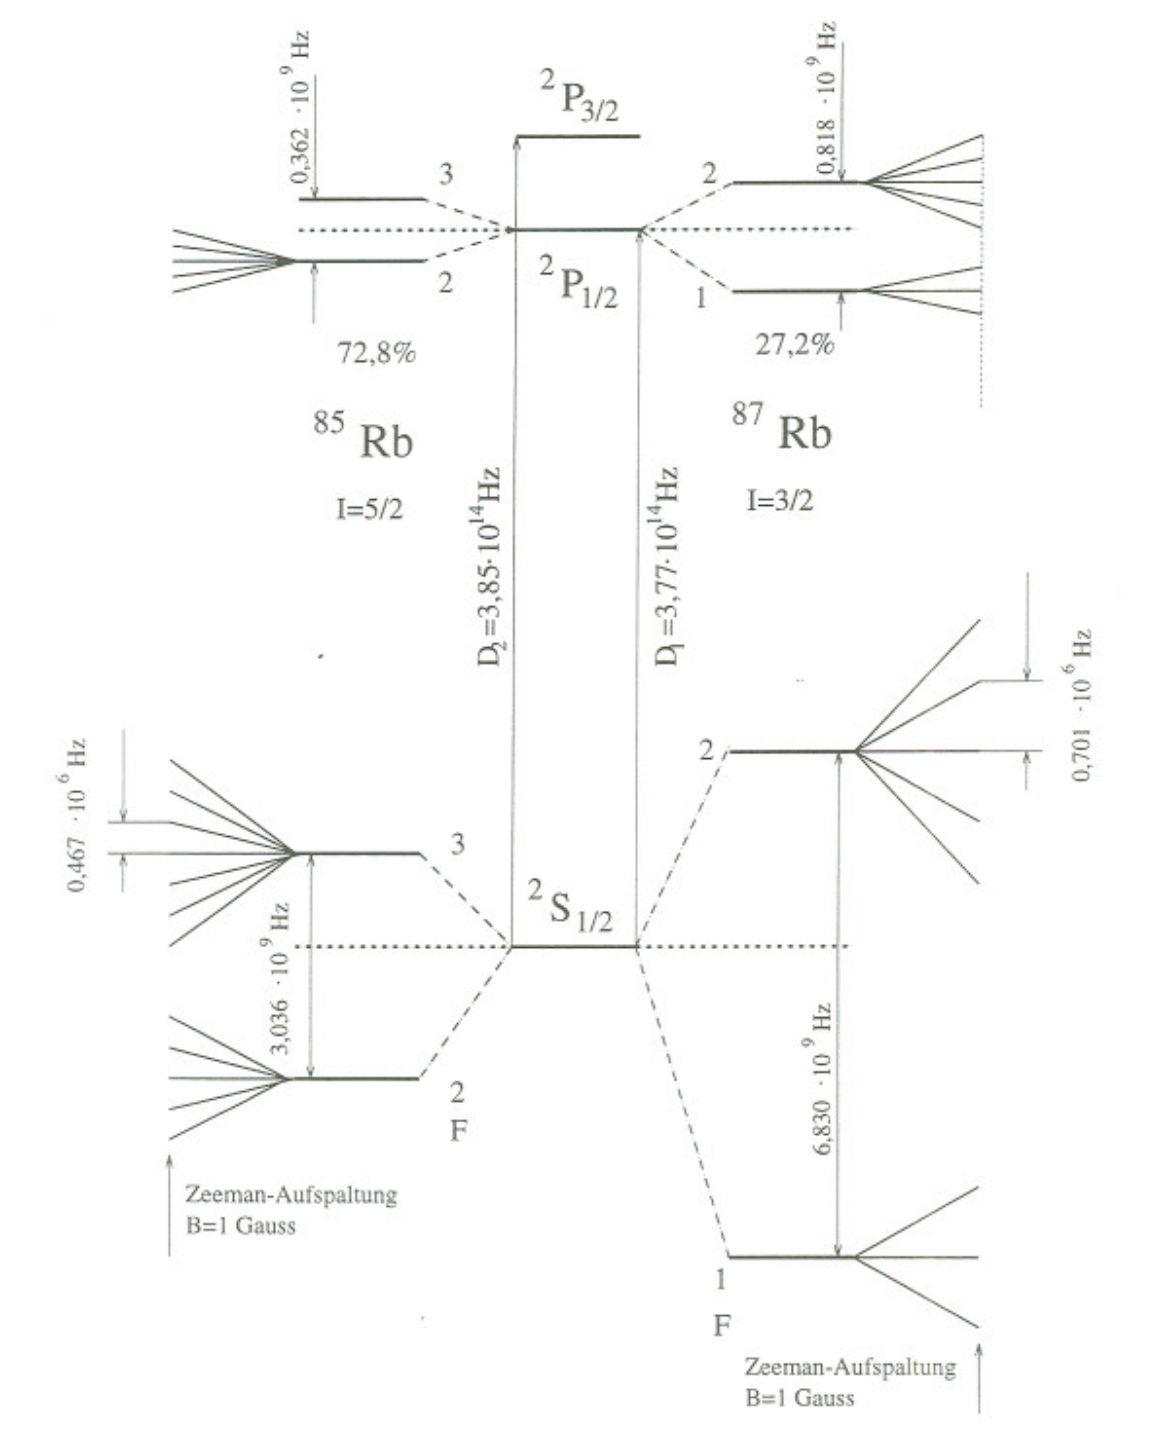
\includegraphics[width=1.0\linewidth]{graphics/hyperfinestructure}
\caption[Hyperfine structure of Rubidium]{The hyperfine structure of the two isotopes of Rubidium used in the experiment. An exemplary Zeeman splitting is included as well. \cite{staatsex}}
\label{fig:hyperfinestructure}
\end{figure}


\subsection{Optical pumping}
\subsection{Larmor precession of the spin}
\subsection{Relaxation processes}
\subsection{The laser diode}
